
\begin{figure*}
     \centering
        \begin{subfigure}[t]{0.49\textwidth}
        \begin{center}
     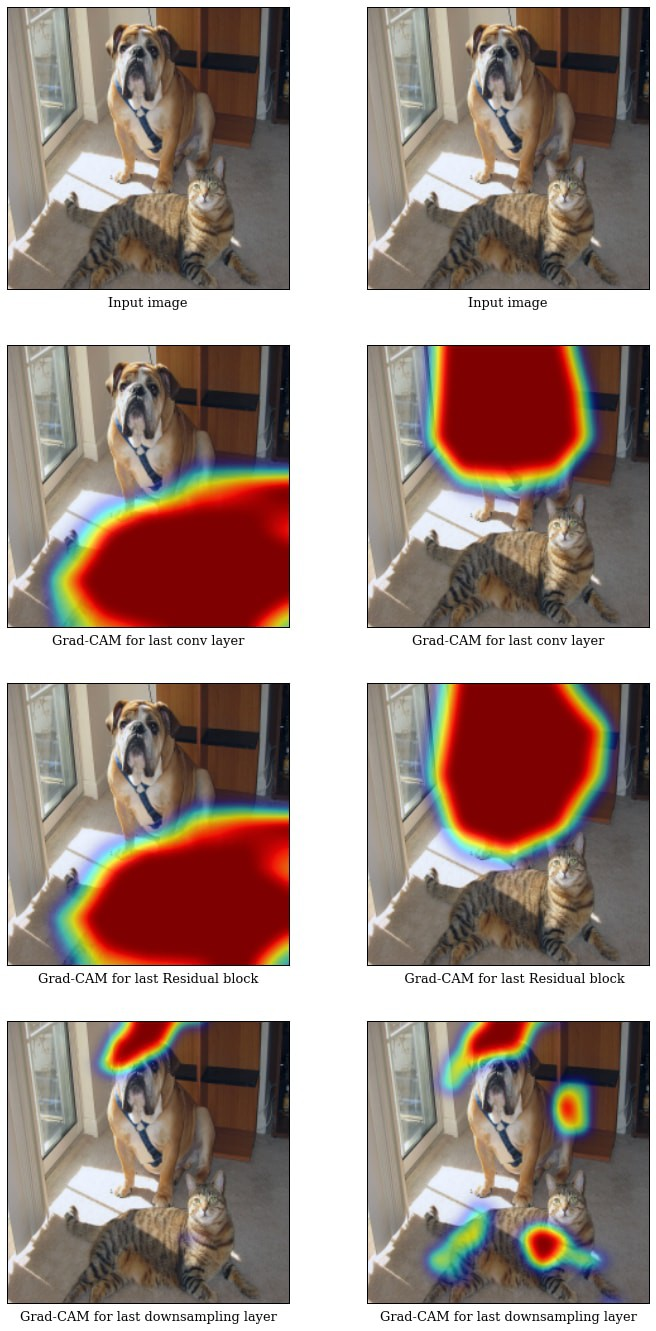
\includegraphics[width=\linewidth]{figures/resnet_200_analysis.jpg}
     \caption{\gcam{}  visualizations for the ResNet-200 layer architecture for 'tiger cat'(left) and 'boxer'(right) category.}
 \end{center}
    \end{subfigure}
    \begin{subfigure}[t]{0.49\textwidth}
        \begin{center}
     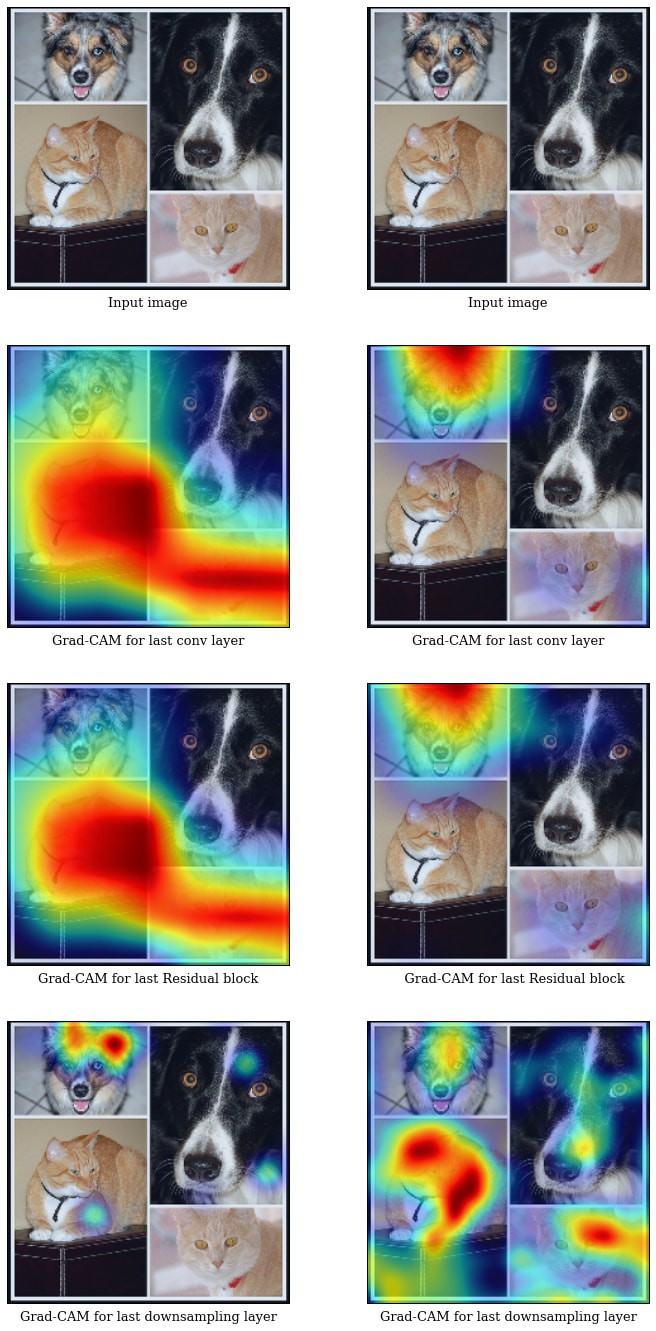
\includegraphics[width=\linewidth]{figures/resnet_200_analysis-2.jpg}
     \caption{\gcam{}  visualizations for the ResNet-200 layer architecture for 'tabby cat'(left) and 'boxer'(right) category.}
        \end{center}
    \end{subfigure}
    \vspace{18pt}
    \caption{We observe that the discriminative ability of \gcam{} significantly reduces as we encounter the downsampling layer.}
     \label{fig:sup_resnet}
\end{figure*}


\vspace{-10pt}
\section{Visual and Textual explanations for Places dataset}\label{sec:sup_text_exp}
\vspace{-15pt}
\reffig{fig:sup_text_explanations} shows more examples of visual and textual explanations (\refsec{sec:text_exp}) for the image classification model (VGG-16) trained on Places365 dataset (\cite{zhou2017places}).



